\documentclass[12pt]{article}
\usepackage{lingmacros}
\usepackage{tree-dvips}
\usepackage{setspace}
\usepackage{hyperref}
\usepackage[nottoc]{tocbibind}
\usepackage{graphicx}
\usepackage{indentfirst}
\usepackage[export]{adjustbox}

%Path relative to the .tex file containing the \includegraphics command
\graphicspath{ {./images/} }
% %Path in Windows format:
% \graphicspath{ {c:/user/images/} }

\title{Rainforest Species Audio detection}
\author{Henry Chang \\Final Project, Machine Learning, Prof. Sven Anderson}
\date{\today}
\doublespace
\begin{document}
\maketitle


\section{Introduction}

\subsection*{Motivation} \small{ 

This project originates from a \href{https://www.kaggle.com/c/rfcx-species-audio-detection/overview}{Kaggle data challenge} hosted by Rainforest Connection, a organization that created a scalable real-time monitoring system for studying and protecting remote ecosystems.  With the prevalence of IoT devices and voice recognition, one can install audio recording devices in natural environment and process the recorded audio with voice recognition techniques to keep tract of wild species activities. The objective of this project is to automate the detection of bird and frog species in tropical soundscape recordings. The challenge comes from the large number of sound sources from the natural environment that would go into the recording, including background noise that varies with weather, sounds of species that is not of interest. High density of overlapping sounds makes the task of species recognition difficult.

}\subsection*{Literature Review} \small{

Traditional methods in audio and image processing uses algorthmic means to extract bird song features. The algorithm design requires human expert to examine the audio data, transform them into different representation and design filters and extractors to capture the sound feature for different species. Bardeli (2010) detects different temporal patterns in frequency bands typical for a species to identify them \cite{BARDELI2010}.

Bird song identification can be seen as a subclass of sound event detection (SED). CNN, which has shown success in similar detection of simple audio features such as keywords, can be directly applicable to species detection \cite{KeywordRecognition}. However, to capture complex temporal data, one often needs to adopt Recurrent Nerual Network (RNN). Convolutional recurrent neural networks (CRNNs), which combines the capacitiy of CNN and RNN, has shown success in SED tasks. By adopting a bidirectional RNN, Adavanne (2017) extends CRNN to a convolutional bidirectional recurrent neural network (CBRNN) for bird song identification. Their work has shown around 90\% accuracy score for cross-validations \cite{RCNN}. 

}\section{Methods}

\subsection*{Data overview}\small{
There are about 4.8k one minute recordings of the rainforest soundscape. Each recording can contain multiple species. Each training example specifies a time window in the recordings where a species appear with a certain type of song type. There are about 4k false positive examples and about 1.1k true positive examples. I will use the true positive examples as they can directly be used for training.}

\begin{figure}[h!]
     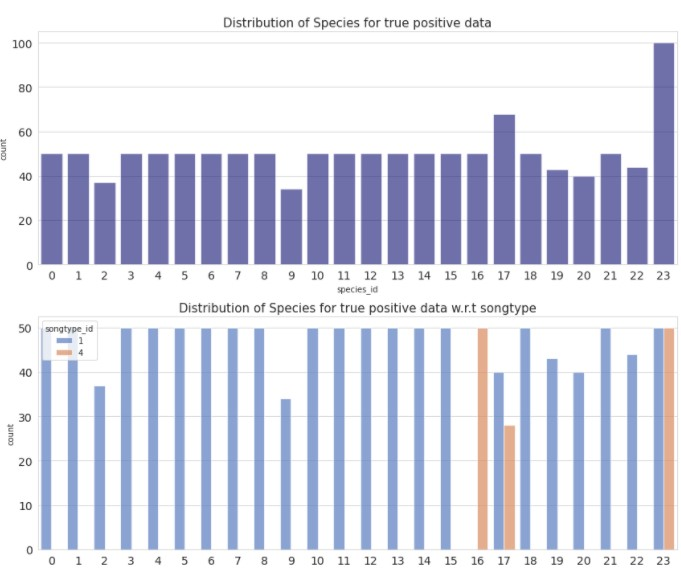
\includegraphics[scale=1, center]{distribution.JPG}
    \caption{Species Distribution}
    \label{fig:distribution}
\end{figure}
  

\small{ The above figure shows that species are mostly evenly distributed, so probabolistic models wouldn't be effective for classification for my task. 
}

\subsection*{Features Preview}

Even though deep neural network automates feature extraction, transforming temporal audio signal into certian representations presents feature in such a way that allows more effective learning. Typically, different species sing in different frequency ranges, so spectrograms of audio signals provide more immediate information for model training. 

\begin{figure}[h!]    
    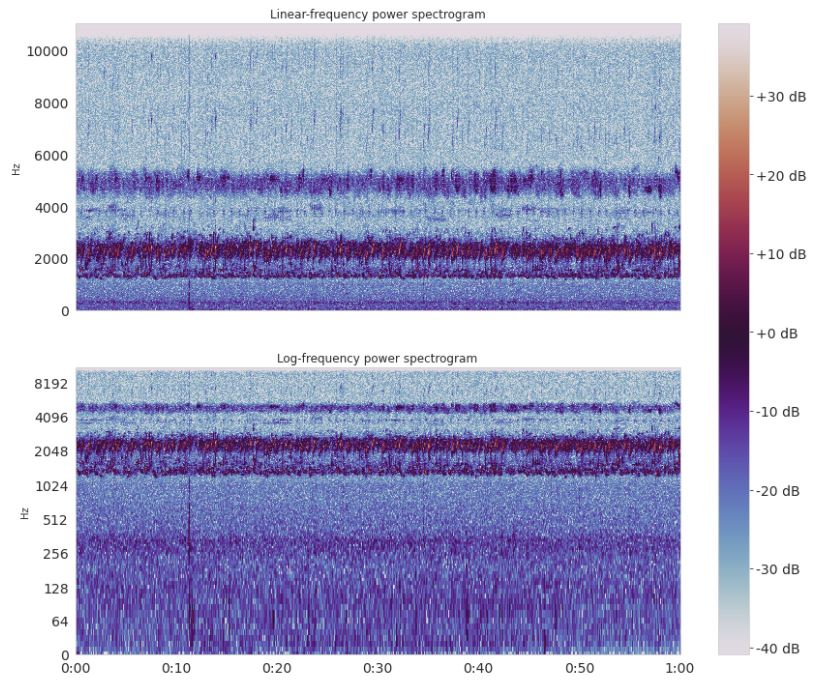
\includegraphics[scale=.8, center]{spectrogram.JPG}   
    \caption{Spectrogram and Log Spectrogram}
    \label{fig:spectrogram}
  \end{figure}

In the above picture, the audio features mostly fall below 6000Hz, so it is useful to view the log the spectrogram to magnify lower frequency ranges and focus on our region of interest. The Mel-spectrogram that captures the perceptual scale that humans hear is also an quite useful representation. In the image below, the frequency range around 400-1k Hz is amplified compared to regular spectrogram. This is helpful since the fundamental frequency of audible features mostly appear in the frequency range of 400-1k Hz. Anything above them could simply be theiry harmonic partial any might as well be neglected. 


\begin{figure}[h!]
    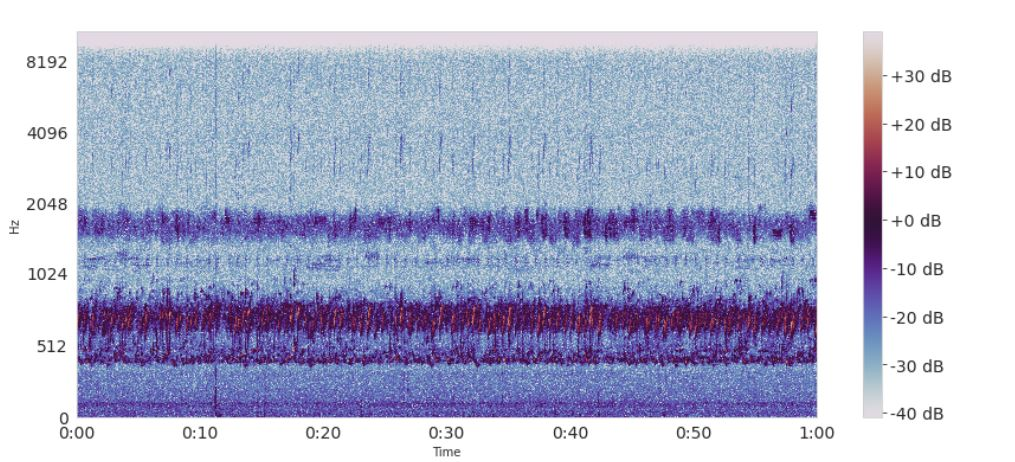
\includegraphics[scale=.7, center]{melspectrogram.JPG}
    \caption{Mel-spectrogram}
    \label{fig:Mel-spectrogram}
\end{figure}

There are other audio features such as zero-crossing rate, spectral centroid, Mel-cepstrum,  Chroma and more. However, since the Mel-spectrogram involves little human processing and diplays audio features in with visual features that can be immediately extracted by nueral networks, we will adopt Mel-spectrogram as the input data for a start. Below is a figure of the Mel-spectrograms for different species. As we can see, a species sings with its temporal patterns in a particular frequency range. The shapes of the individual envelopes are also specifc to specifies.


\begin{figure}[h!]
    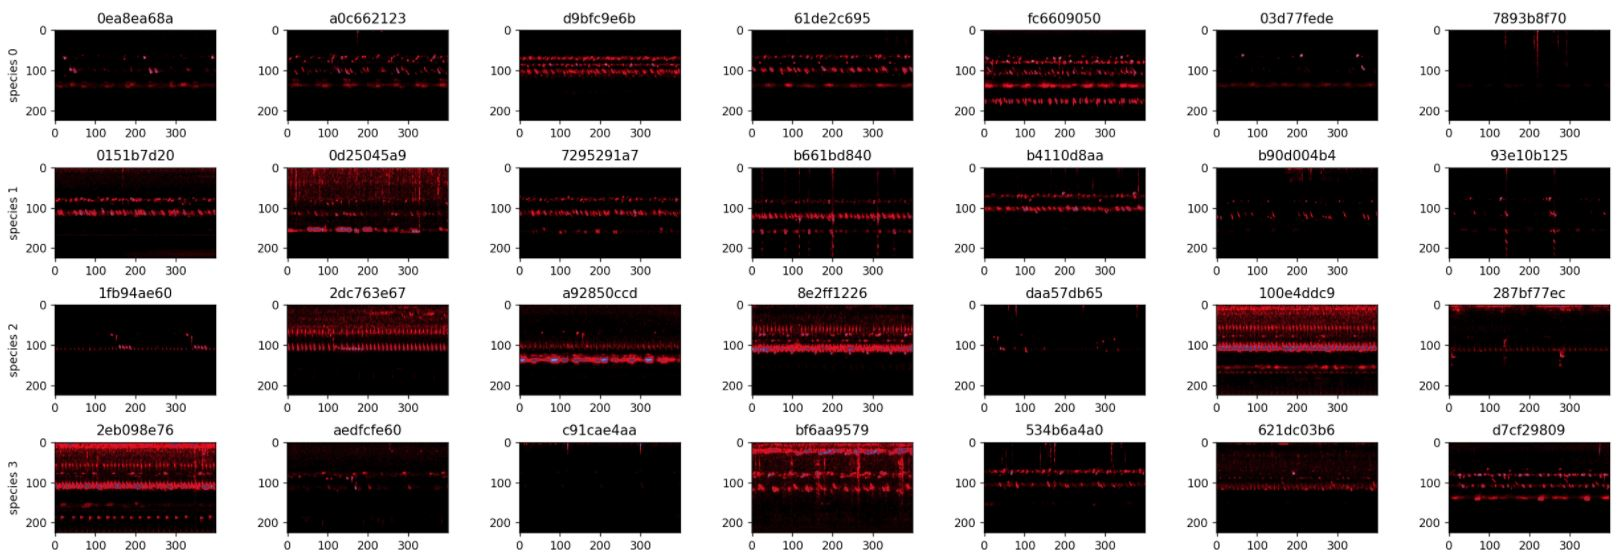
\includegraphics[scale=0.5, center]{species.JPG}
    \caption{Mel-spectrogram}
    \label{fig:Mel-spectrogram}
\end{figure}

\newpage

\section{Methods}
Based on our literature review and data preview, I will start by using CNN to identify the shapes characteristic of specifies inside spectrograms. The project will then be extended to RCNN to capture temporal patterns. 

I experimented with running a basic CNN (with 2 convolutional, 1 max pooling and 1 Dense layer) on the input spectrograms. This network even though small, has shown success in reconizing keywords with high accuracy \cite{KeywordRecognition}. To feed the spectrograms into the network, the annotated windows are sliced into fixed size of 0.26s, the duration of the smallest annotated window. The networked learned with increasing accuracy and decreasing loss. However, given the evaluation format of Kaggle dataset, I need to submit the prediction of species given a particular audio file that is one minute long. 

My intuition is to slice the test data into small pieces. Predict the probabilities of species in each slice, take their maximums and use them for the prediction of the full audio file. However, transforming all the slices and making predictions on them took too long (more than 6 hrs) for Colab and Kaggle engine to run for the entire dataset of around 2k test files (the evaluation strictly checks that every testfile is predicted), so my implementation hasn't been able to display result on the testing data. See this \href{https://colab.research.google.com/drive/1p0j7Wd9AU0Hdjy4hyJS1wBnhpe-etGQ8?usp=sharing}{notebook} for my basic CNN implementation.

Instead, I will look closely at the similar example of a Kaggle notebook by Yosshi999 (2020) that performs a baseline transfer learning using Resnet50 \cite{resnet50TPU} with a sequntial layer head to covert features for classification. The Resnet50 is a Deep CNN, so its result can also shed light on the capacitiy of applying CNN to species detection. 

Yosshi999's implementation cuts 6 seconds around the annotation of where a species appear as input for training. To avoid overfitting, Dropout layer and data augmentation are used. Data augmentation includes adding Gaussian noise, random brightness, mixup \cite{Mixup} and SpecAugment \cite{SpecAugment}. After training for 15 epoch with batch size of 64, the training ended with a loss of  .15 and .85 metric score.  The testing data gives a .77 score for the "label-weighted label-ranking average precision" used by the data challege. 

\begin{figure}[h!]
    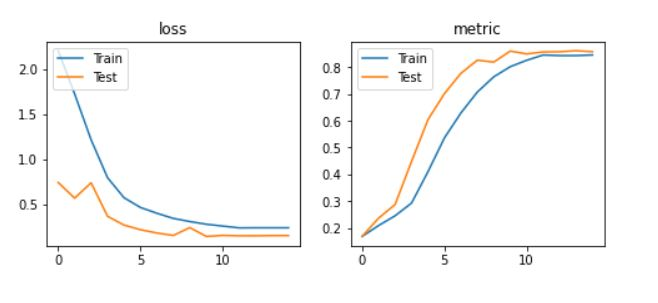
\includegraphics[center]{learnCurve.JPG}
    \caption{Learning History}
    \label{fig:learningCurve}
\end{figure}

\newpage

\section{Conclusion}
Overall, the applicaton of Resnet50 has shown progress of learning for the first 10 epochs but then starts to platue. The .77 test score is decent but is far away from human level identification. The .7 difference between training and testing score means that there are still space for generalization on unseen data. 

\section{Future Direction}
To narrow the difference between training and testing score and improve on the current application of Resnet50, we can extract the other audio features mentioned ealier as input into the network. 

However, since CNN have translational invariance, the temporal repetition of the same species singing woudn't be learned by CNN as effectively. Intead, models that has shown success in speech recognition can be applied to our tasks of species recognition. We can capture the relation between time sequences of spectrogram by incorporating the concept of memory. Therefore, Recurrent Neural Network (RNN) and Long Short-Term Memory network (LSTM) are immediately great candidates. Since songs of species aren't as complex as human speech, networks with attention mechanism might not be extra helpful, and simple RNN should do the work. The next step of this project will be using simple RNN or RCNN models for species detection. 
\newpage
\bibliographystyle{plain}
\bibliography{ref.bib}
\end{document}